\documentclass[table]{beamer}
\useoutertheme[subsection=false]{smoothbars}
\usecolortheme{beaver}

\usepackage{xcolor}
\usepackage[utf8]{inputenc}
\usepackage[french]{babel}
\usepackage{graphicx}
\usepackage{hyperref}
\usepackage{tikz}
\usetikzlibrary{shapes.geometric, arrows}

\definecolor{links}{HTML}{F0132D}

\hypersetup{colorlinks, linkcolor=structure!50!red, urlcolor=links}

\setbeamercolor{caption name}{fg=structure!50!red}
\setbeamerfont{alerted text}{series=\bfseries}
\setbeamercolor{itemize item}{fg=structure!50!red}

\makeatletter
\newcommand*{\rom}[1]{\expandafter\@slowromancap\romannumeral #1@}
\makeatother

\tikzstyle{memory} = [rectangle, rounded corners, minimum width=3cm, minimum height=1cm,text centered, draw=black, fill=red!30]
\tikzstyle{registers} = [rectangle, rounded corners, minimum width=3cm, minimum height=1cm, text centered, draw=black]
\tikzstyle{empty} = [rectangle, minimum width=3cm, minimum height=1cm, text centered]
\tikzstyle{arrow} = [thick,->,>=stealth]

\title{Horloge numérique}
\subtitle{Systèmes numériques}
\author{Oscar Garnier \and Yannis Kedadry \and Antoine Anastassiades}
\institute{\'Ecole Normale Supérieure -- Département d'Informatique}
\date{24 janvier 2023}

\begin{document}

	\frame{\titlepage}

	\begin{frame}
		\frametitle{Sommaire}
		\tableofcontents
	\end{frame}

	\section{L'assembleur}
	\begin{frame}
		\frametitle{Correspondance syntaxe-addresses}
		\def\arraystretch{1.5}
		\begin{tabular}{c*{5}{p{0.15\textwidth}}}
			&31\hfill20&19\hfill15&14\hfill10&9\hfill5&4\hfill0\\
			\cline{2-6}
			R&\multicolumn{1}{|c|}{immédiat}&\multicolumn{1}{|c|}{rs2}&\multicolumn{1}{|c|}{rs1}&\multicolumn{1}{|c|}{rd}&\multicolumn{1}{|c|}{opcode}\\
			\cline{2-6}
			I&\multicolumn{2}{|c|}{immédiat}&\multicolumn{1}{|c|}{rs}&\multicolumn{1}{|c|}{rd}&\multicolumn{1}{|c|}{opcode}\\
			\cline{2-6}
			U&\multicolumn{3}{|c|}{immédiat}&\multicolumn{1}{|c|}{rd}&\multicolumn{1}{|c|}{opcode}\\
			\cline{2-6}
		\end{tabular}
	\end{frame}

	\begin{frame}
		\frametitle{Les opcodes}
			\def\arraystretch{2.5}
			\begin{tabular}{p{0.08\textwidth}||c*{8}{p{0.08\textwidth}}}
				& 000 & 001 & 010 & 011 & 100 & 101 & 110 & 111 \\
				\cline{1-9}
				00 & Addi & & Srli & Srai & Slli & Andi & Ori & Xori \\
				\cline{1-9}
				01 & Add & Sub & Srl & Sra & Sll & And & Or & Xor \\
				\cline{1-9}
				10 & Lw & Sw & & Beq & Bne & Blt & Blti & Bge \\
				\cline{1-9}
				11 & Lui & Auipc & Jal & Jalr & & & Slt & Slti \\
			\end{tabular}
	\end{frame}

	\section{Microprocesseur}
	\begin{frame}
		\frametitle{Schéma du microprocesseur}
		\begin{figure}
			\centering
			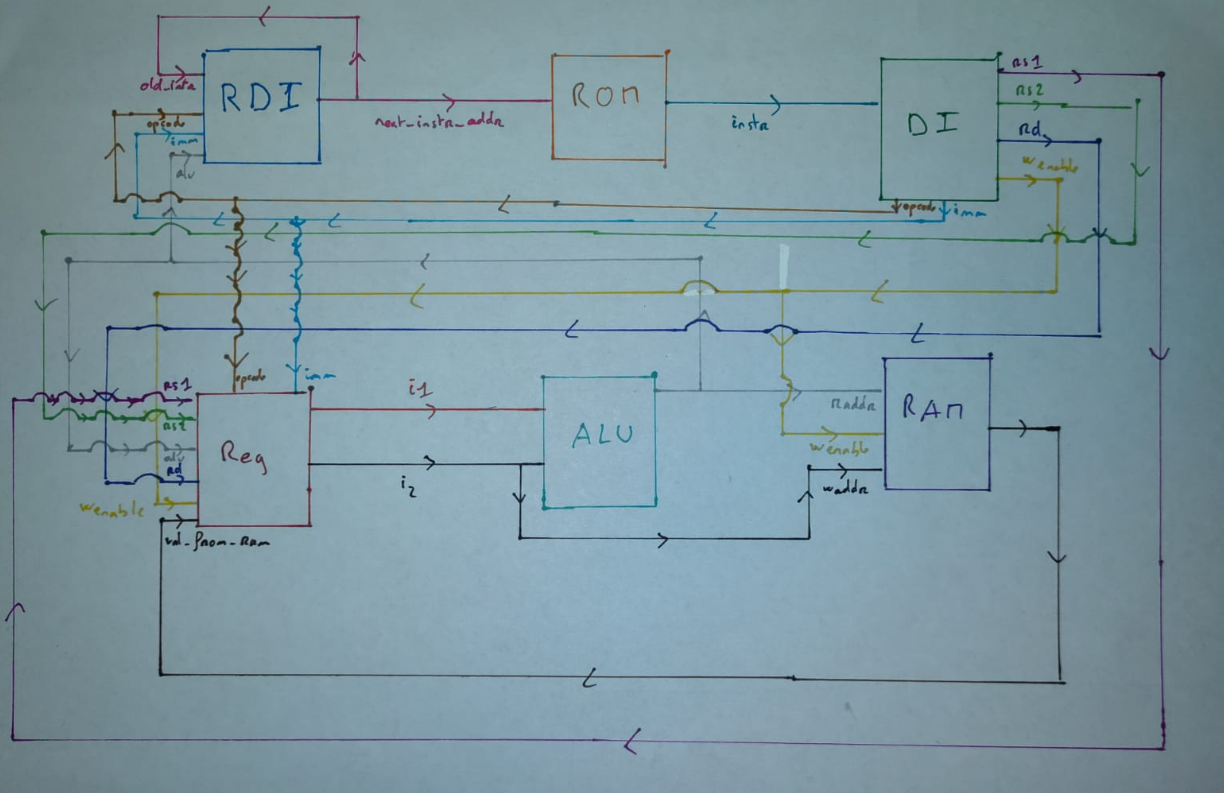
\includegraphics[width=\textwidth]{microproc_schema.png}
		\end{figure}
	\end{frame}

	\section{Le simulateur de netlist}
	\begin{frame}
		\frametitle{Le simulateur de netlist}
		\begin{figure}
			\centering
			\begin{tikzpicture}
				\node (net) [empty] {};
				\node (sim) [registers, right of=net, xshift=4cm] {simulateur};
				\node (stdout) [empty, right of=sim, xshift=4cm] {};
				\node (clk) [empty, below of=net] {-{}-clk};
				\node (nstep) [empty, below of=clk] {-n nstep};
				\node (rom) [empty, below of=nstep] {-rom $*.i$};

				\draw [arrow] (net) -- node[anchor=south] {.net} (sim);
				\draw [dashed,->] (clk) -| (sim);
				\draw [dashed,->] (nstep) -| (sim);
				\draw [dashed,->] (rom) -| (sim);
				\draw [arrow] (sim) -- node[anchor=south] {stdout} (stdout);

			\end{tikzpicture}
		\end{figure}
	\end{frame}

	\section{Clock}
	\begin{frame}
		\frametitle{A l'initialisation}
		\begin{figure}
		\centering
		\begin{tikzpicture}[node distance=2cm]
			\node (x14) [registers] {x14: sec};
			\node (dot) [empty, below of=x14] {\dots};
			\node (x19) [registers, below of=dot] {x19: yr};
			\node (ram) [memory, right of=dot, xshift=2cm] {RAM};
			\node (dbdb) [registers, below of=x19] {Double-Dabble};

			\draw [arrow] (ram) |- node[anchor=south] {0x2} (x14);
			\draw [arrow] (ram) -- node[anchor=north] {0x\(i\)} (dot);
			\draw [arrow] (ram) |- node[anchor=north] {0x7} (x19);
			\draw [arrow] (x19) -- (dbdb);
		\end{tikzpicture}
		\end{figure}
	\end{frame}

	\begin{frame}
		\frametitle{Pendant un cycle}
		\begin{figure}
		\centering
		\begin{tikzpicture}[node distance=2cm]
			\node (x13) [registers] {x13: sec};
			\node (dot) [empty, below of=x13] {\dots};
			\node (x0) [registers, below of=dot] {x0: yr};
			\node (ram) [memory, right of=x13, xshift=5cm] {RAM};

			\draw [arrow] (ram) -- node[anchor=south] {0x1: si 1 : + 1} (x13);
			\draw [arrow] (x13) -- node[anchor=east] {\emph{overflow}} (dot);
			\draw [arrow] (dot) -- node[anchor=east] {\emph{overflow}} (x0);
		\end{tikzpicture}
		\end{figure}
	\end{frame}

	\begin{frame}
		\frametitle{Double-Dabble}

		\only<1>
		{\begin{center}
			\def\arraystretch{1.5}
			\begin{tabular}{|c|c|c|c|c|c|c|c|c|c|c|c|c|c|}
				\multicolumn{13}{c}{}&\multicolumn{1}{c}{15}\\
				\cline{1-4} \cline{6-9} \cline{11-14}
				0&0&0&0&&0&0&0&0&&1&1&1&1\\
				\cline{1-4} \cline{6-9} \cline{11-14}
			\end{tabular}
		\end{center}}
		\only<2>
		{\begin{center}
			\def\arraystretch{1.5}
			\begin{tabular}{|c|c|c|c|c|c|c|c|c|c|c|c|c|c|}
				\multicolumn{14}{c}{}\\
				\cline{1-4} \cline{6-9} \cline{11-14}
				0&0&0&0&&0&0&0&1&&1&1&1&\cellcolor{black!50}x\\
				\cline{1-4} \cline{6-9} \cline{11-14}
			\end{tabular}
		\end{center}}
		\only<3>
		{\begin{center}
			\def\arraystretch{1.5}
			\begin{tabular}{|c|c|c|c|c|c|c|c|c|c|c|c|c|c|}
				\multicolumn{14}{c}{}\\
				\cline{1-4} \cline{6-9} \cline{11-14}
				0&0&0&0&&0&0&1&1&&1&1&\cellcolor{black!50}x&\cellcolor{black!50}x\\
				\cline{1-4} \cline{6-9} \cline{11-14}
			\end{tabular}
		\end{center}}
		\only<4>
		{\begin{center}
			\def\arraystretch{1.5}
			\begin{tabular}{|c|c|c|c|c|c|c|c|c|c|c|c|c|c|}
				\multicolumn{8}{c}{}&\multicolumn{1}{c}{+3}&\multicolumn{4}{c}{}\\
				\cline{1-4} \cline{6-9} \cline{11-14}
				0&0&0&0&&0&1&1&1&&1&\cellcolor{black!50}x&\cellcolor{black!50}x&\cellcolor{black!50}x\\
				\cline{1-4} \cline{6-9} \cline{11-14}
			\end{tabular}
		\end{center}}
		\only<5>
		{\begin{center}
			\def\arraystretch{1.5}
			\begin{tabular}{|c|c|c|c|c|c|c|c|c|c|c|c|c|c|}
				\multicolumn{14}{c}{}\\
				\cline{1-4} \cline{6-9} \cline{11-14}
				0&0&0&0&&1&0&1&0&&1&\cellcolor{black!50}x&\cellcolor{black!50}x&\cellcolor{black!50}x\\
				\cline{1-4} \cline{6-9} \cline{11-14}
			\end{tabular}
		\end{center}}
		\only<6>
		{\begin{center}
			\def\arraystretch{1.5}
			\begin{tabular}{|c|c|c|c|c|c|c|c|c|c|c|c|c|c|}
				\multicolumn{3}{c}{}&\multicolumn{1}{c}{1}&\multicolumn{4}{c}{}&\multicolumn{1}{c}{5}&\multicolumn{4}{c}{}\\
				\cline{1-4} \cline{6-9} \cline{11-14}
				0&0&0&1&&0&1&0&1&&\cellcolor{black!50}x&\cellcolor{black!50}x&\cellcolor{black!50}x&\cellcolor{black!50}x\\
				\cline{1-4} \cline{6-9} \cline{11-14}
			\end{tabular}
		\end{center}}

	\end{frame}

	\part{}
	\begin{frame}[plain] % The optional argument 'plain' hides the headline and footline
		\frametitle{Ce qui peut être amélioré}
		\begin{itemize}
			\item Double-Dabble en dur
			\item Meilleur Jal
			\item Découper la RAM en octets
		\end{itemize}
	\end{frame}
		
\end{document}
